%===============================================================
%   A Brief History of the Deflection of Light
%===============================================================
\section{A Brief History of the Deflection of Light}

In the beginning, there was Newtonian gravity. For nearly 400 years, Newton's Laws of Motion and Gravity accurately predicted the movements of celestial bodies. The nature of light up until the late 19th and early 20th century was still a mystery, as well as to its relationship with gravity. Henry Cavendish in 1784 \citep{Cavendish:2011ts} and later Johann von Soldner in 1804 \citep{Jaki:1978wc}, posited that light could behave similarly as massive particles and be deflected in the vicinity of a strong gravitational potential. This deflection angle was computed to be

\begin{equation}
\alpha_\mathrm{Newton} = \frac{2GM}{c^2b}
\end{equation}

\noindent where $M$ is the mass of the object and $b$ is the impact parameter, or distance of closest approach to $M$.

However, Albert Einstein's relativity does not allow for massive objects and light to travel through spacetime in a similar manner, as light particles always have a spacetime interval of $ds^2=0$ (light always travels at $c$ in all reference frames). Thus, light will follow geodesics unique to those of massive particles when influenced by the bending of space and time by a massive object \citep{Einstein:1911rf}. Using the Schwarzchild metric for a point mass and following the weak field limit (i.e., $GM/c^2r$ \textless \textless\ 1 along the entire trajectory), one obtains an alternative result for the deflection of light:

\begin{equation}
\alpha_\mathrm{Einstein} = \frac{4GM}{c^2b} =  2\alpha_\mathrm{Newton}.
\label{intro:eqn:deflection}
\end{equation}

This postulate of general relativity provided the first opportunity to test the controversial theory. The best measuring man in England, Arthur Eddington, was intrigued by the German physicist's theory, and despite facing barriers put in place to prevent collusions with enemy scientists during the time of World War I, he collaborated with Einstein and devised an experiment to measure the deflection of background stars by the Sun during the 1919 solar eclipse. Einstein predicted a deflection of 1.74 seconds of arc of the stars in the background Hyades cluster. On May 29, two teams in Sobral, Brazil and the island of Principe of the coast of Africa measured a deflection of $1.98\pm0.16$" (see Figure~\ref{intro:fig:eclipse}) and $1.6\pm0.40$", respectively, both well within two sigma of the prediction by Einstein and far ruling out the Newtonian prediction of 0.87". When the article was published on November 6th, 1919, Einstein became a world-wide celebrity overnight \citep{Dyson:1920zl}.

\begin{figure}
\centering
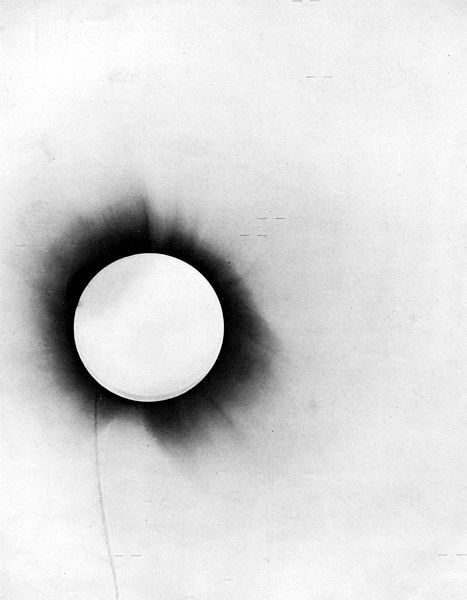
\includegraphics[width=0.8\textwidth]{Intro/1919_eclipse_negative.jpg}
\caption[Photometric plates from the 1919 solar eclipse]{From \citet{Dyson:1920zl}, original caption: ``From the report of Sir Arthur Eddington on the expedition to verify Albert Einstein's prediction of the bending of light around the sun. In Plate 1 is given a half-tone reproduction of one of the negatives taken with the 4-inch lens at Sobral. This shows the position of the stars, and, as far as possible in a reproduction of this kind, the character of the images, as there has been no retouching. A number of photographic prints have been made and applications for these from astronomers, who wish to assure themselves of the quality of the photographs, will be considered as as far as possible acceded to."}
\label{intro:fig:eclipse}
\end{figure}

%===============================================================
%   Extragalactic Gravitational Lensing
%===============================================================

\section{Extragalactic Gravitational Lensing}

Fritz Zwicky and Albert Einstein both suggested that galaxies rather than stars would make for much stronger gravitational lenses \citep{Zwicky:1937yq,Einstein:1936cl}. And indeed, later in the 20th century, astronomers began discovering this deflection of light, or gravitational lensing as it became known, by extragalactic sources. In rare cases, the deflection can be strong enough such that the light from the background source can travel multiple paths around the deflecting, or lensing, object, thus creating multiple images of the background source. In 1979, the ``Twin Quasar" was discovered -- two quasars located unusually close together in the sky, both behind a massive foreground galaxy, shown in Figure~\ref{intro:fig:quasar}. Due to the similar redshifts and spectra of the quasars, it was deduced that they were lensed images of the same background quasar.

\begin{figure}
\centering
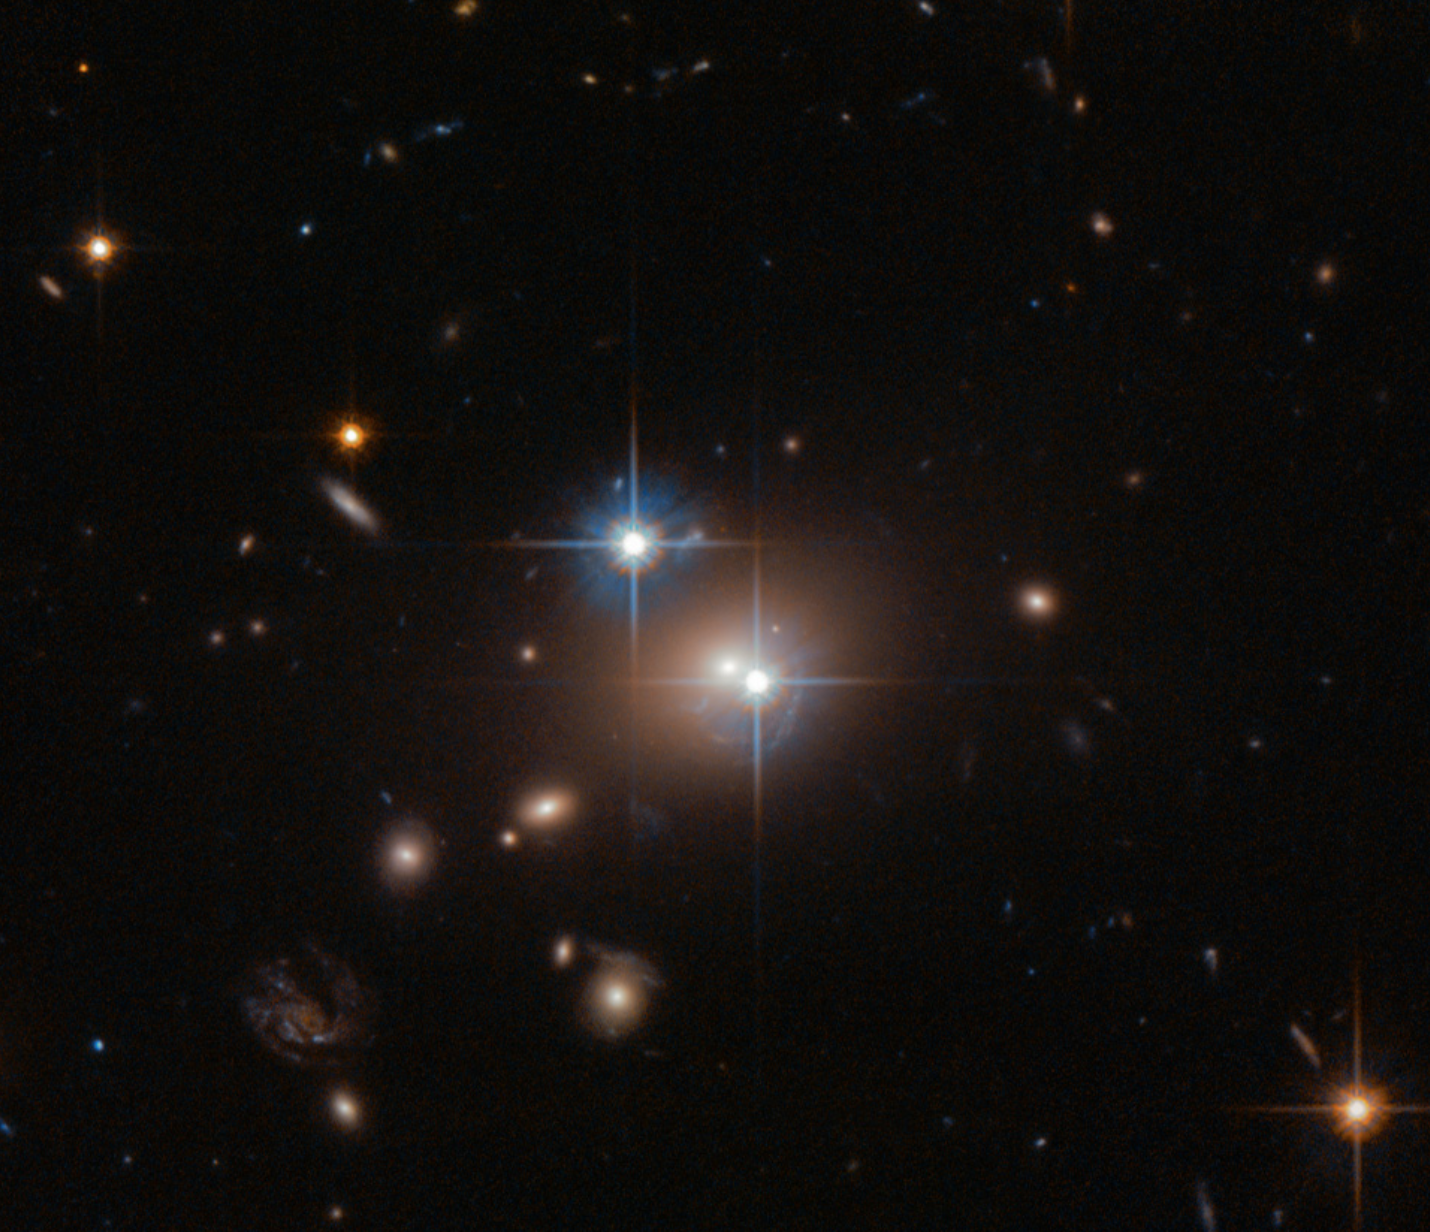
\includegraphics[width=0.8\textwidth]{Intro/twin_quasar.png}
\caption[\hst\ image of the Twin Quasar]{{\it Hubble Space Telescope} (\hst) image of the famous Twin Quasar. From  ``Seeing double". ESA/Hubble Picture of the Week. Retrieved 30 November 2017.}
\label{intro:fig:quasar}
%http://www.spacetelescope.org/images/potw1403a/
\end{figure}

Galaxy clusters are the most massive gravitationally-bound objects in the Universe, consisting of hundreds of galaxies clustered within a virial radius of on the order of a megaparsec. Zwicky used galaxy clusters to hypothesize the existence of an invisible mass in galaxy clusters, as the velocity dispersion of the galaxies suggested the total masses of these clusters to be $400\times$ higher than the mass implied by the star light of the galaxies \citep{Zwicky:1937yq}. This dark matter, as it has come to be known, has been proven time and time over to exist. The mass of a typical galaxy cluster consists of only $\sim1\%$ that of the baryonic component of the cluster members and nearly $\sim90\%$ dark matter. The remaining $\sim9\%$ is contained in the 10 million degree intergalactic medium, which would have been ``invisible" to Zwicky, but today is visible with Xray telescopes.

Certain galaxy clusters are capable of behaving as gravitational lenses, provided they are massive and have an ideal mass profile, which we will discuss later. Finding these lenses; however, would prove quite difficult as they would have to be very bright and highly magnified to be detected, being as they were billions of light years away, and distorted significantly to be seen as obvious signs of lensing. This work would have been impossible on photographic plates as faint lensed galaxies could easily be mistaken for cluster member galaxies or optical defects in the plate. Ultimately, it took the sensitivity and resolution of the CCD camera that allowed for the discovery of gravitational lenses. And indeed, the first spectroscopically-confirmed cluster lensed galaxy was discovered in the field of Abell 370 in 1986 \citep{Soucail:1988kx,Soucail:1987sf,Soucail:1987rz}, shown in Figure~\ref{intro:fig:a370}. Interestingly, we will learn more about this cluster using sophisticated gravitational lens modeling in Chapter~\ref{chap:hff_clusters}.

\begin{figure}
\raisebox{50pt}{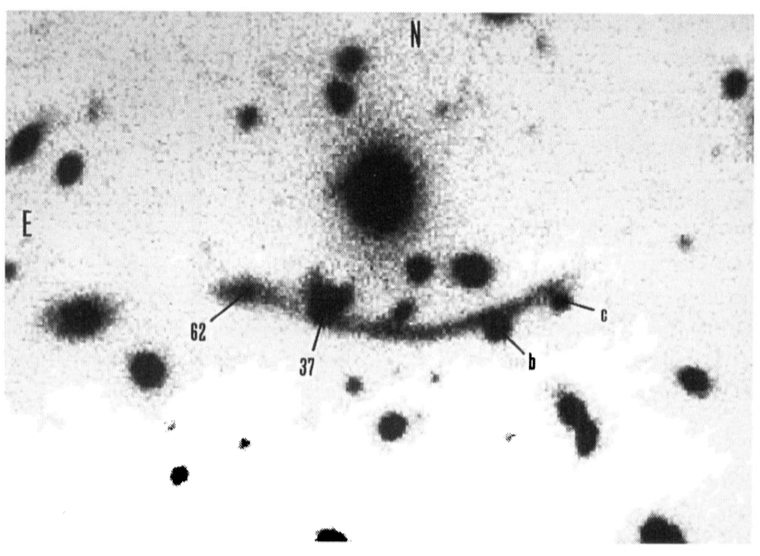
\includegraphics[width=0.35\textwidth, trim=0 10pt 0 0, clip, angle=-28]{Intro/soucail88.png}}
\includegraphics[width=0.55\textwidth, trim=100pt 200pt 100pt 200pt, clip]{Intro/a370_hff.jpg}
\caption[Images of Abell 370 -- the first cluster lens]{Left: From \citet{Soucail:1988kx}, original caption: ``CCD frame of the giant arc in A370. This picture was obtained by J.L.~Prieur at the prime focus of the 3.60m Canada-France-Hawaii telescope on October 25th, 1987. The CCD was a $640\times1024$ RCA2: scale 0.2"/pixel -- seeing 0.7", with an exposure time of 10 minutes in white light. Note the shape of the object \#37, which was already suspected based on its spectrum \citet{Soucail:1987sf}", meaning that since the object is not at the cluster redshift, but indeed behind it and being lensed into a fantastic arc. Right: 140-orbit \hst\ image of Abell 370 from the Hubble Frontier Fields Director's Discretionary Program. From ``The last of the Frontier Fields -- Abell 370. STScI. Retrieved 30 November 2017.}
% https://www.spacetelescope.org/images/heic1711a/
\label{intro:fig:a370}
\end{figure}

%===============================================================
%   Gravitational Lensing Theory
%===============================================================

\section{Gravitational Lensing Theory}

\subsection{The one-dimensional lensing equation}

\begin{figure}
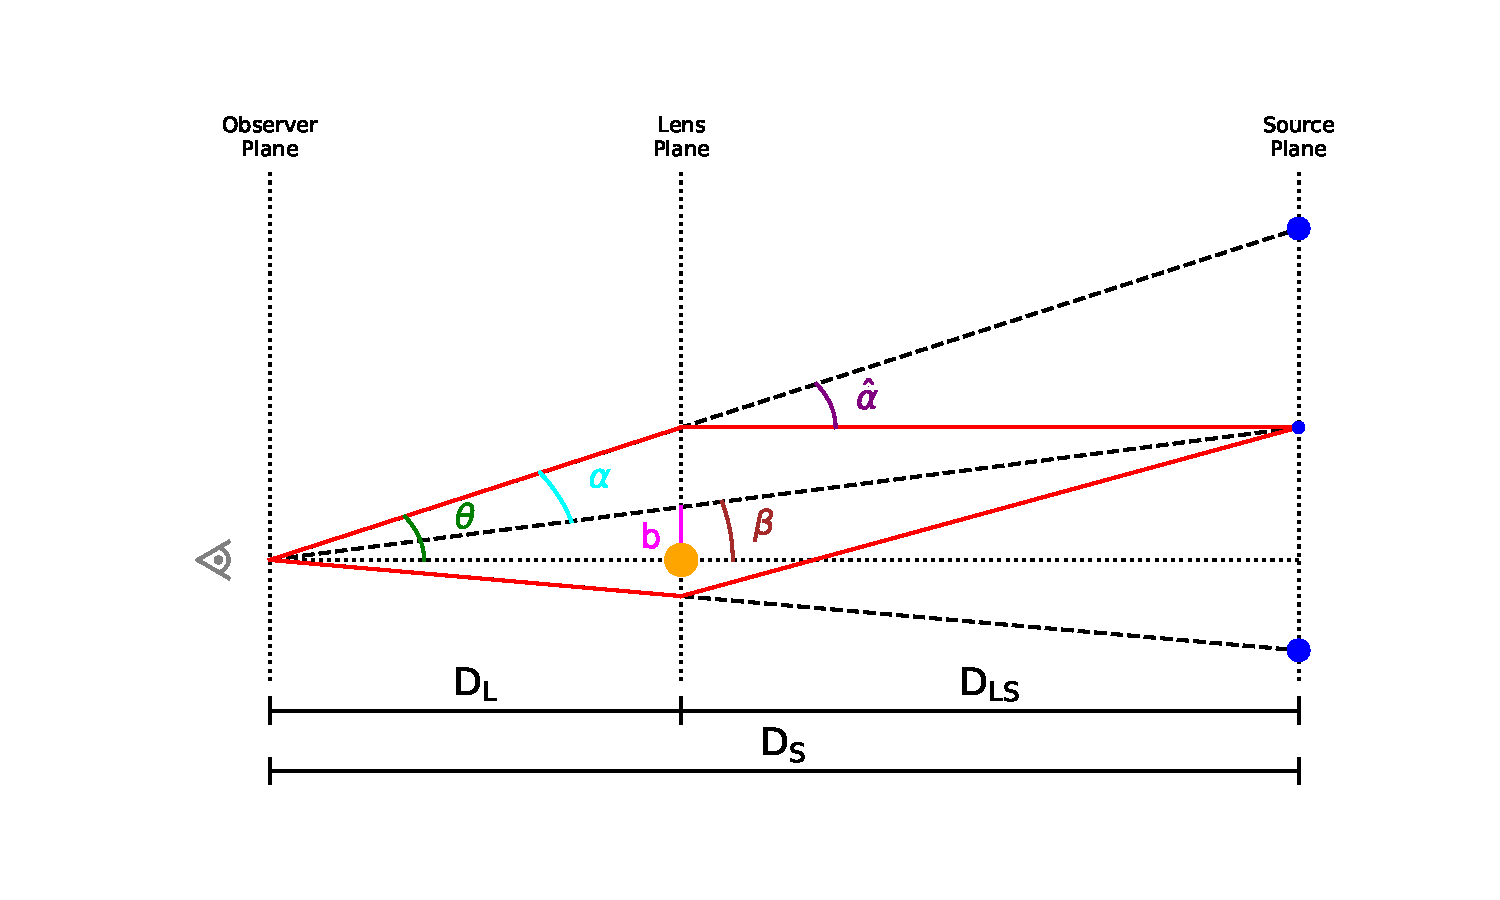
\includegraphics[width=\textwidth, trim=75pt 75pt 75pt 75pt]{Intro/lens_diagram.pdf}
\caption[Diagram of gravitational lensing parameters]{Diagram showing the definitions of angles and distances used for deriving the lens equation.}
\label{intro:fig:diagram}
\end{figure}

Since the distances of between the lens, source, and observer are much larger than the size of the lens itself, it is safe to use the ``thin lens approximation" popular in optics where we assume an instantaneous deflection of the light on a plane of mass created by the lens. Therefore, we envision the geometry of the lensing as shown in Figure~\ref{intro:fig:diagram}. The distances $\dl$, $\ds$, and $\dls$ are the angular diameter distances between the observer-lens, observer-source, and lens-source, respectively. We define the angle between the lens and source in the observer's frame to be $\beta$ and the angle between the lens and of the apparent position of the image of the source to be $\theta$. The angle $\hat\alpha$ is the deflection angle computed by Einstein in (\ref{intro:eqn:deflection}). Using the small-angle approximation, we can write

\begin{equation}
\theta \ds = \beta \ds + \hat\alpha \dls,
\end{equation}

\noindent and after rearranging, we get that

\begin{equation}
\beta(\theta) = \theta - \frac{\dls}{\ds} \hat\alpha,
\end{equation}

\noindent known as the lensing equation. Here, we have redefined $\beta$ as a function of $\theta$ as every image will map to only a single source, which should be fairly intuitive. We can also define another variable

\begin{equation}
\alpha \equiv  \frac{\dls}{\ds} \hat\alpha,
\label{intro:eqn:dlsds}
\end{equation}

\noindent which is the angular offset between the image and the source at the location of the observer. While $\hat\alpha$ will always remain constant for a given impact parameter, the observed deflection depends on the geometry of the lensing system, i.e., the relative distances to the source and lens.

\subsection{Lensing in two-dimensions and magnification}
\label{intro:sec:magnification}

We have so far been working in one dimension considering positions of sources and images on singular axes. The solutions hold for any axisymmetrical lens; however, in nature, we must consider that mass distributions are more complex, and thus will cause a dependence on position angle of the source rather than purely the impact parameter, $\theta\dl$. In the simple case shown in Figure~\ref{intro:fig:diagram}, our one-dimensional lens has produced two point source images. This is also true if we extend the solution to two-dimensions, except in the instance where source is directly behind the lens ($\beta=0$). In this case, the solution is a circle (or ring) of radius

\begin{equation}
\theta = \alpha = \frac{\dls}{\ds} \frac{4GM}{c^2} \frac{1}{\theta \dl}
\end{equation} 

\noindent from which we define the Einstein radius as

\begin{equation}
\theta_E^2 \equiv \frac{4GM}{c^2} \frac{\dls}{\dl\ds}.
\label{intro:eqn:einstein_radius}
\end{equation}

\subsection{Lens mapping}

Most sources in the Universe are not point sources and can be magnified, in that the solid angle subtended by their images is larger than that of the source. The exact definition of the magnification is the ratio of these solid angles,
$\mu \equiv \Delta \theta/\Delta \beta$. We can also treat lensing as a mathematical transformation of the shape of a source into its observed images. We can transform the lens equation into a transformation matrix

\begin{equation}
A_{ij} = \frac{\partial \beta_{ij}}{\partial \theta_{ij}} = \delta_{ij} - \frac{\partial{\alpha_{i}}}{\partial{\theta_{j}}} = 
	\begin{bmatrix}
		1-\kappa-\gamma_1 & \gamma_2 \\
		\gamma_2 & 1-\kappa+\gamma_1
	\end{bmatrix},
\end{equation}

\noindent where we have defined the new terms

\begin{align}
\kappa &= \frac{1}{2} \left(\frac{\partial{\alpha_{1}}}{\partial{\theta_{1}}}+\frac{\partial{\alpha_{2}}}{\partial{\theta_{2}}}\right) = \frac{1}{2} \nabla_{ij} \alpha_{ij} = \frac{\Sigma}{\Sigma_{crit}} \label{intro:eqn:kappa} \\
\gamma_1 &= \frac{1}{2} \left(\frac{\partial{\alpha_{1}}}{\partial{\theta_{1}}}-\frac{\partial{\alpha_{2}}}{\partial{\theta_{2}}}\right) \\
\gamma_2 &= \frac{\partial{\alpha_{1}}}{\partial{\theta_{2}}} = \frac{\partial{\alpha_{2}}}{\partial{\theta_{1}}} \\
\gamma^2 &= \gamma_1^2 + \gamma_2^2
\end{align}

\noindent with $\Sigma$ representing the projected surface mass density of the lens plane, with critical surface mass density equal to

\begin{equation}
\Sigma_\mathrm{crit} = \frac{c^2}{4\pi G} \frac{\ds}{\dls\dl}.
\end{equation}

\noindent The formation of multiple and/or highly distorted images, occurs when $\kappa>1$. There are two parts of (\ref{intro:eqn:kappa}) required for lensing, a massive lens ($\Sigma$) and the proper geometrical alignment ($\Sigma_\mathrm{crit}$).

The magnification map can be determined by taking the inverse determinant of the transformation matrix:

\begin{equation}
\mu^{-1} = |\det A| = |(1-\kappa)^2 - \gamma^2|.
\end{equation}

\noindent It is possible for the magnification to be smaller than one (i.e., demagnified images) as well as become infinite. However, the area in the image plane where this occurs is infinitesimally small, so infinite magnifications fall on lines called critical curves. The eigenvalues of $A$ tell us where these lines occur:

\begin{align}
1-\kappa-\gamma &= 0 \\
1-\kappa+\gamma &= 0.
\end{align}

\noindent These describe the tangential and radial critical curves in the image plane, respectively. These are the lines of symmetry between image pairs, reflected either tangentially or radially. Image pairs will have opposite parity; they are mirrors of one another. We can use the lens equation to map these curves to the source plane, producing caustics that inform us on the number of images the lens will produce. The number of images must always be odd, with two additional images being formed for each caustic the source falls within. Often times one of these images is highly demagnified and/or lies behind the bright lens, thus is not always observed and why there are reports of ``double" or ``quad" configurations in the literature. Typical image configurations and their respective source locations are shown in Figure~\ref{intro:fig:image_config}.

For the remainder of this work, we will refer to ``strong" gravitational lensing as the phenomenon in which lensing results in multiple and/or highly-distorted images of the background source.

\begin{figure}
\centering
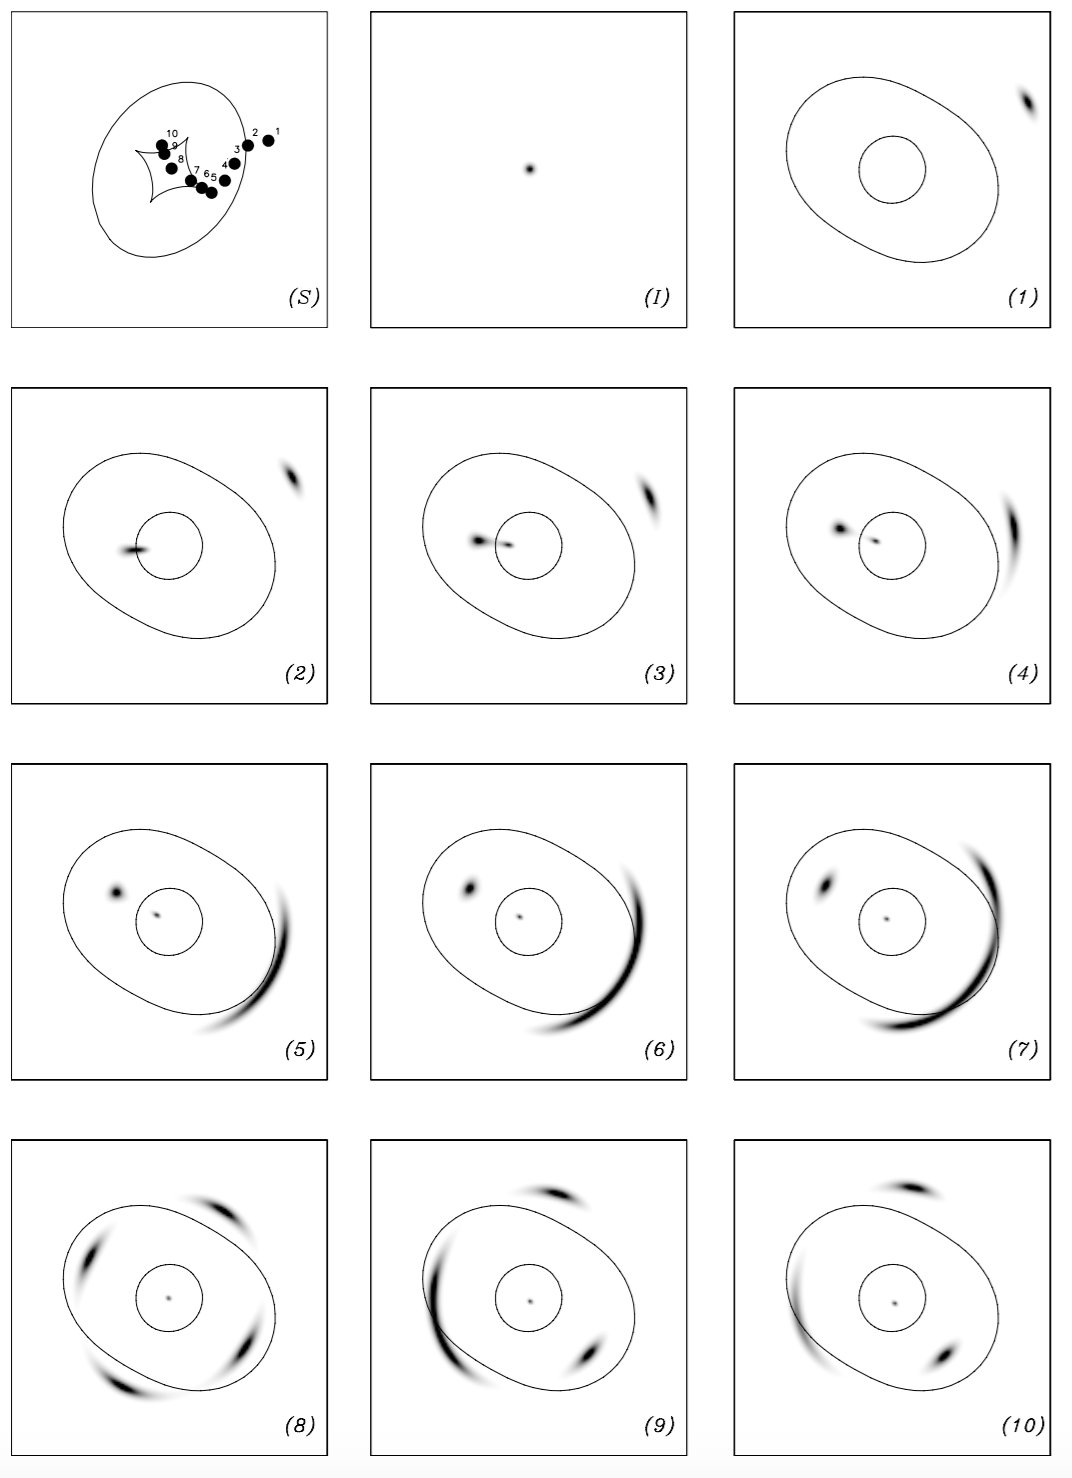
\includegraphics[height=0.8\textheight]{Intro/image_config.png}
\caption[Strong lensing caustics, critical curves, and multiple image configurations]{From \citet{Kneib:2011qy}, original caption: ``Multiple-image configurations produced by a simple elliptical mass distribution. The panel (S) shows the caustic lines in the source plane and the positions numbered 1 to 10 denote the source position relative to the caustic lines. The panel (I) shows the image of the source without lensing. The panels (1) to (10) show the resulting lensed images for the various source positions. Certain configurations are very typical and are named as follows: (3) radial arc, (6) cusp arc, (8) Einstein cross, (10) fold arc."}
\label{intro:fig:image_config}
\end{figure}

\section{Strong gravitational lens modeling}

\subsection{First-order approximation: Einstein radius}

As we found in \S~\ref{intro:sec:magnification}, sources which are almost perfectly aligned with the lens will produce an Einstein ring. By assuming that the lens is axisymmetric, we can determine the total mass within this ring from (\ref{intro:eqn:einstein_radius}), which yields

\begin{equation}
M(<\theta_E) = \pi (\theta_E \dl)^2 \Sigma_\mathrm{crit}.
\label{intro:eqn:einstein_mass}
\end{equation}

Figure~\ref{intro:fig:einstein_ring} shows examples of nearly perfect Einstein rings where this approximation can be made. Typical values for $\theta_E$ in clusters are on the order of $\sim$15", translating to physical scales on the order of a few hundred kiloparsecs. All other estimates for masses based on astronomical observables (ex., X-ray, Sunyaev-Zel'dovich effect, galaxy dynamics, weak lensing, galaxy counts, etc.) are sensitive to the masses at much larger radii ($\sim$1 Mpc). Thus, strong lensing provides a unique estimate for the masses at the very cores of clusters. In conjuction with other techniques, strong lensing can be used to measure the mass-concentration relationship of galaxy clusters, which helps inform on their formation history.

\begin{figure}
\centering
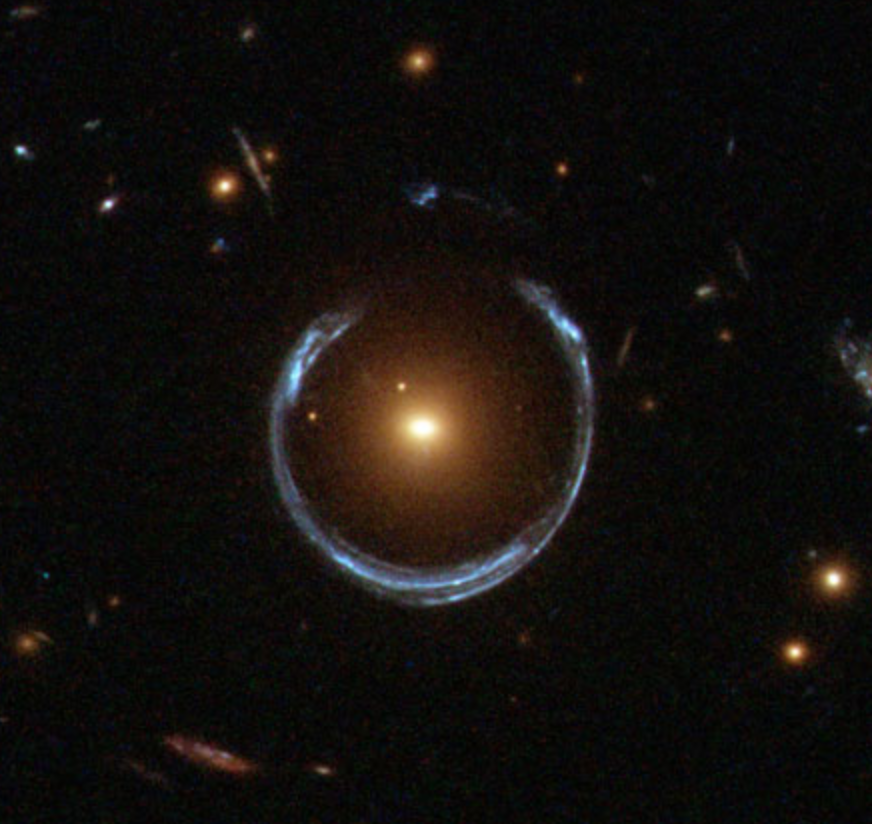
\includegraphics[height=0.3\textheight]{Intro/einstein_ring_1.png}
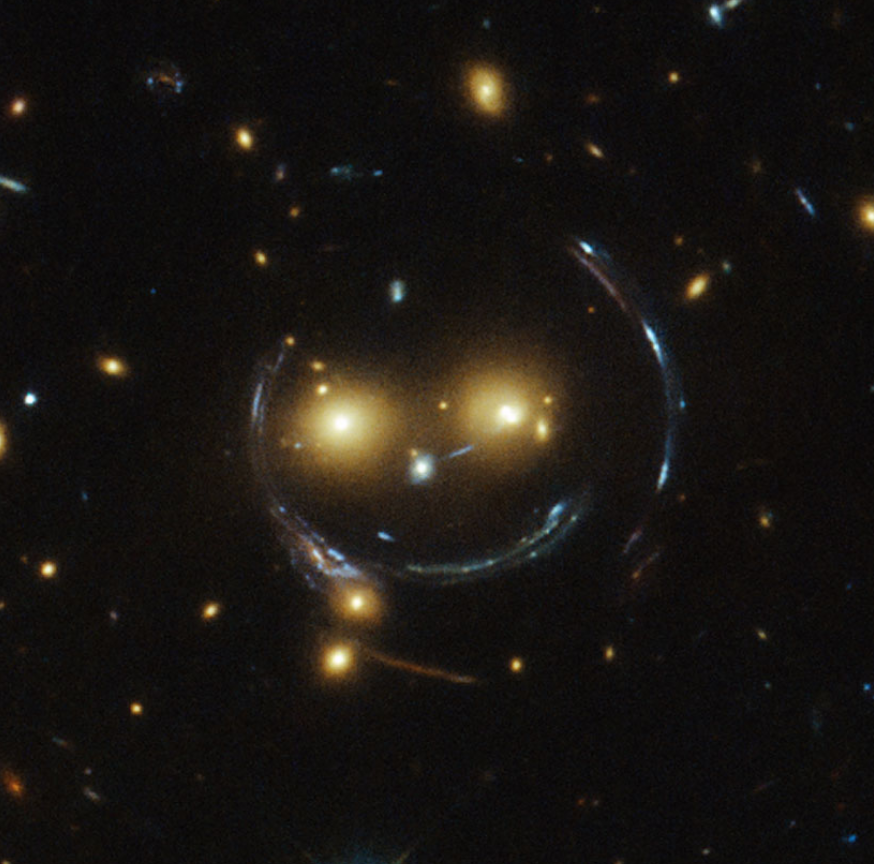
\includegraphics[height=0.3\textheight]{Intro/einstein_ring_2.png}
\caption[\hst\ Einstein Rings]{Two famous Einstein rings imaged with the \hst. (Left): LRG~3-757 nearly forms a perfect ring around the massive elliptical galaxy. (Right): Galaxy cluster SDSS~J1038+4849 forms a pseudo-Einstein ring with partial rings formed from several lensed background sources.}
% http://apod.nasa.gov/apod/ap111221.html
% https://en.wikipedia.org/wiki/Einstein_ring#cite_note-NASA-20150210-6
\label{intro:fig:einstein_ring}
\end{figure}

However, galaxy clusters are not necessarily axisymmetric and contain a lot of substructure in the form galaxies, which perturb the local lensing potential. While it is a close approximation, a precise determination of the mass distribution requires more careful modeling which can take into account shape and substructure of the cluster.

\subsection{Lens modeling}

A more precise model of the lensing mass can be achieved using the positions of multiple images. By finding a deflection field that maps all multiple images to a single position in the source plane, an estimate for the mass can be computed using (\ref{intro:eqn:kappa}). Using more sets of multiple images will help to further constrain the deflection field at different radii. After examining (\ref{intro:eqn:einstein_mass}), we see that $\Sigma_\mathrm{crit}$ is linear with $\alpha$ and thus scales in the same manner as (\ref{intro:eqn:dlsds}). Having a range of redshifts from different sources will produce a range of Einstein radii, which will help to constrain the slope of the mass distribution (such as the cluster in the right image of Figure~\ref{intro:fig:einstein_ring}).

The general approach to lens modeling involves finding the mass distribution which creates the deflection field that best reproduces the observed image configuration. These approaches fall into two categories: ``parametric" and ``non-parametric". The former involves defining the surface mass density of the cluster and its galaxies in terms of physically-motivated potentials such as an isothermal sphere or a Navarro, Frenk, and White profile \citep[NFW; ][]{Navarro:1997qa}. These methods rely heavily on the assertion that ``light traces mass." Therefore, the total mass is scaled by the total light from the galaxy, usually following the empirical fundamental plane of luminosity, radius, and velocity dispersion of elliptical galaxies \citep{Gudehus:1973kq}. ``Non-parametric" methods allow for more flexible characterization of the mass distribution by employing either a pixelized array of masses or a grid of radial basis functions that can each fluctuate in total mass to affect the localized deflection near multiple images as well as the overall shape of the mass distribution. Generally, this method does not force the notion that galaxies must have mass, but allows for the image configurations to constrain the masses on smaller-scale structures as needed to reproduce the lensing effect.

The modus operandi of this author is a parametric method established by the \texttt{LENSTOOL} software \citet{Jullo:2007lr} and embodies lens modeling inquiry presented in this dissertation. Therefore, detailed discussions of the variants of non-parametric methods is beyond the scope of this work.

\subsubsection{Bayesian statistics and model optimization}

Regardless of the modeling method, nearly all have settled on a exercising a Bayesian approach, where optimizing a model depends not only on its fitness, but also information about the parameters obtained a priori. The Bayes' theorem is defined

\begin{equation}
P(\vec{p} | D ) = \frac{P(\vec{p}) P(D | \vec{p} ) }{P(D)}
\label{intro:eqn:bayes}
\end{equation}

\noindent where $D$ are the observed data, and $\vec{p}$ contains the parameters of the model. Let us break down each component of (\ref{intro:eqn:bayes}):

\begin{itemize}
\item $P(\vec{p} | D )$: The posterior probability distribution -- the probability of the model given the data. In this instance, the data are the locations of the multiple images along with their distance from the lens and observer (i.e., redshift).
\item $P(\vec{p})$: The prior. This term is the a probability that a particular model is accurate based on {\it a priori} information.
\item $P(D | \vec{p} )$:  The likelihood of getting the data given the parameters of the model. Non-Bayesian modeling focuses this term in optimization (i.e., maximum likelihood estimation) and de-regulates the prior.
\item $P(D)$: The evidence. This term is the probability that a particular model is valid independent of all other variables, which effectively acts as Occam's razor: ``All things being equal, the simplest solution tends to be the best one." The evidence normalizes the posterior probability distribution.
\end{itemize}

Bayes' theorem can easily be applied to strong lens modeling once we define a likelihood function to include in our optimization. The likelihood function will take the form

\begin{equation}
P(D | \vec{p} ) = \prod_{i=1}^N \frac{1}{  \prod_{j=1}^{n_i} \sigma_{ij} \sqrt{2\pi} } \exp^{-\frac{\chi_i^2}{2}},
\label{intro:eqn:likelihood}
\end{equation}

\noindent where $N$ is the number of sources, $n_i$ is the number of images of each source $i$, and $\sigma_{ij}$ is the measurement error image $j$ of source $i$. By minimizing $\chi^2$, we will produce the maximum likelihood model. As stated earlier, our goal in lens modeling is to find the which finds a solution with the smallest scatter between the source positions mapped to each of its images. Defining the likelihood in this manner is called source plane optimization. While this still solves the lens equation, it is not ideal as the exact position of the sources are unknown to the observer. The more appropriate method would be image plane optimization, which involves an extra step of ray tracing the source position of each image back out to the image plane and measuring the scatter of the predicted images. However, this second step is much more computationally intensive due to the ray tracing, which is required because the lens equation is not invertible. The $\chi_i^2$ function for each source $i$ will then take the form

\begin{equation}
\chi^2 = \sum_{j=1}^{n_i} \frac{[\theta_\mathrm{obs}^j - \theta^j (\vec{p})]^2}{\sigma_{ij}^2},
\label{intro:eqn:chi2}
\end{equation}

\noindent where $\theta^j (\vec{p})$ is the predicted image position ray traced to the observed image position $\theta_\mathrm{obs}^j$. Examining this equation further, we can see that image plane optimization will ensure that models which produce additional images than those observed are likely to be rejected as they will produce much higher $\chi^2$ than models with fewer images (smaller $n_i$).

It should be noted that this method could be improved by including additional lensing information in the optimization, such as magnification, time delays, and/or flexion (i.e., shape), which could be added in quadrature to (\ref{intro:eqn:chi2}). Some lens modeling methodologies do include these terms; however, for this work, we will only consider image positions as the primary constraint.

\subsubsection{Computational methods}

The \texttt{LENSTOOL} software utilizes a Markov Chain Monte Carlo (MCMC) to sample parameter space to determine the shape of the posterior probability distribution. In the MCMC burn-in phase, ``walkers" of models are initialized with a set of parameters randomly sampled from the current posterior probability distribution. At the first stage, the likelihood has not been sampled yet, so it is not included in the initial determination of the posterior. This is done by replacing the likelihood in Bayes' theorem (\ref{intro:eqn:bayes}) with the term $P(D | \vec{p} )^\lambda$, where $\lambda$ is a ``cooling" parameter. At the beginning, $\lambda=0$, so in the analogy to thermodynamics, the model selection is ``hot" and samples from a wide range of values in parameter space, ensuring that the MCMC can find a global maximum likelihood. The posterior probability for each walker is computed, and a new $\vec{p}$ is selected for each walker and given a probability to jump based on the ratio of the posterior probability of the current position and the new position. Walkers will tend to jump to higher posterior probabilistic positions in parameter space as the chain continues to form, all while $\lambda$ is slowly increasing from 0 to 1 at a rate chosen to insure a smooth convergence towards a colder posterior probability distribution. After $\lambda=1$, the burn-in phase is complete and the changes are re-initialized from the last position in parameter space for all the walkers. Using the full Bayes' theorem, a new MCMC runs to sample the posterior probability distribution.

\subsection{Data for cluster lensing}

Lens modeling has benefited from the imaging CCDs aboard the {\it Hubble Space Telescope} (\hst). The high sensitivity and high resolution allow for easier detection and identification of multiple image systems to be used in the modeling. The first remarkable instance of using \hst\ for cluster lensing of Abell 2218 \citep{Kneib:1996kb} imaged with the Wide Field Planetary Camera 2 (WFPC2) is shown in Figure~\ref{intro:fig:lensing_clusters}. 

\begin{figure}
\centering
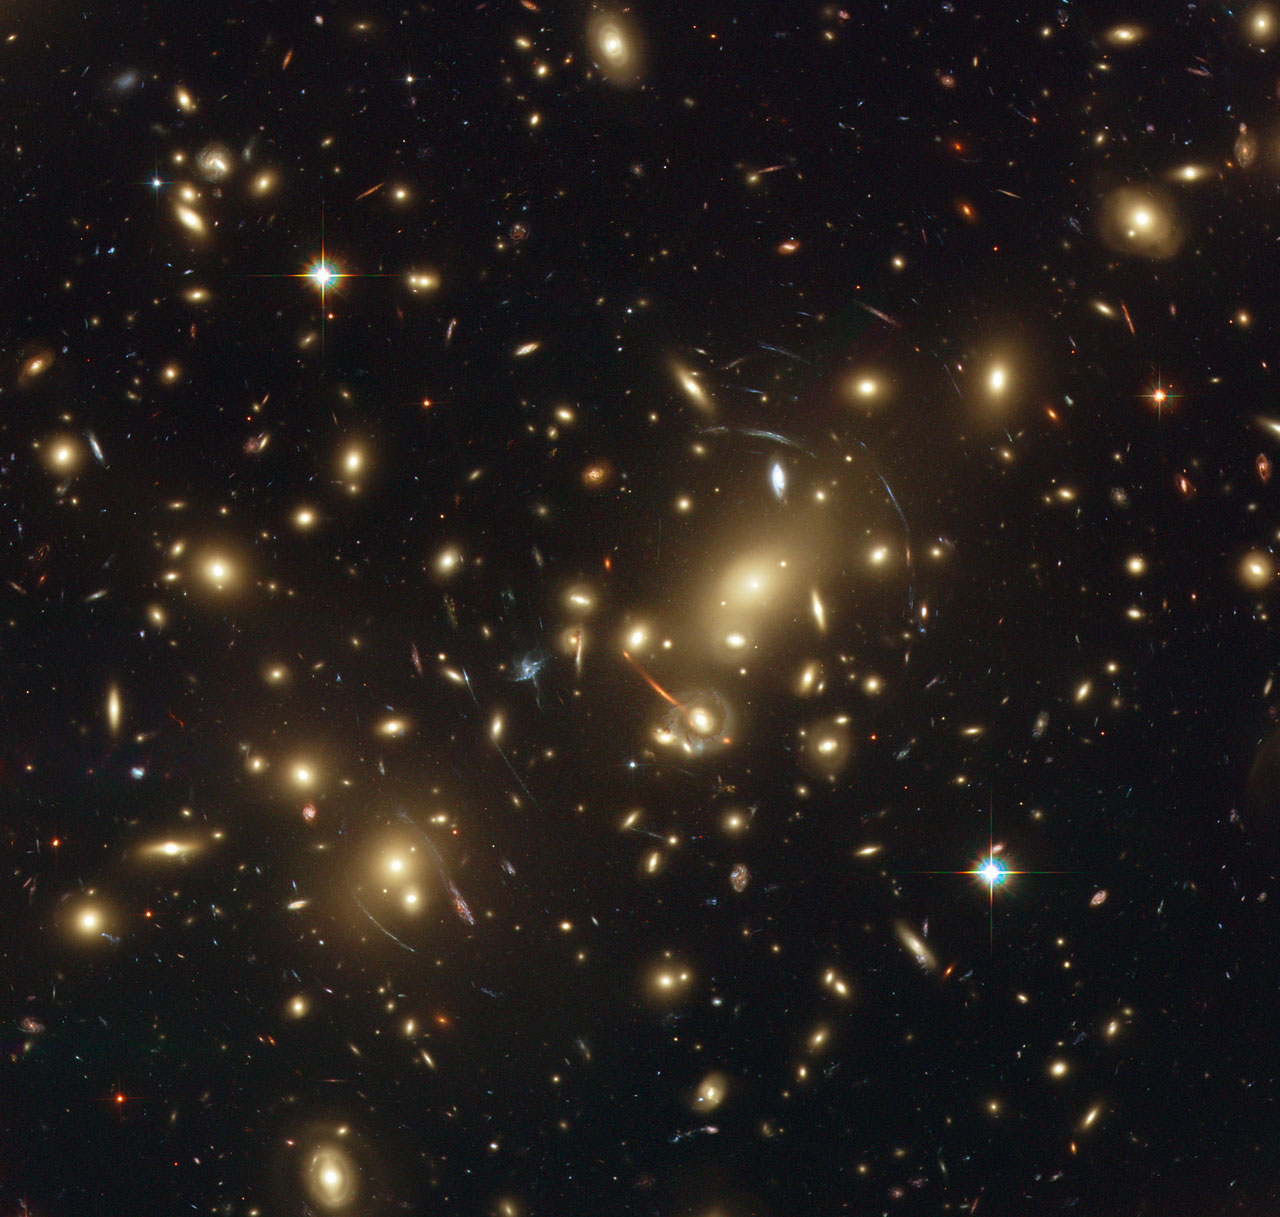
\includegraphics[height=0.3\textheight]{Intro/a2218.jpg}
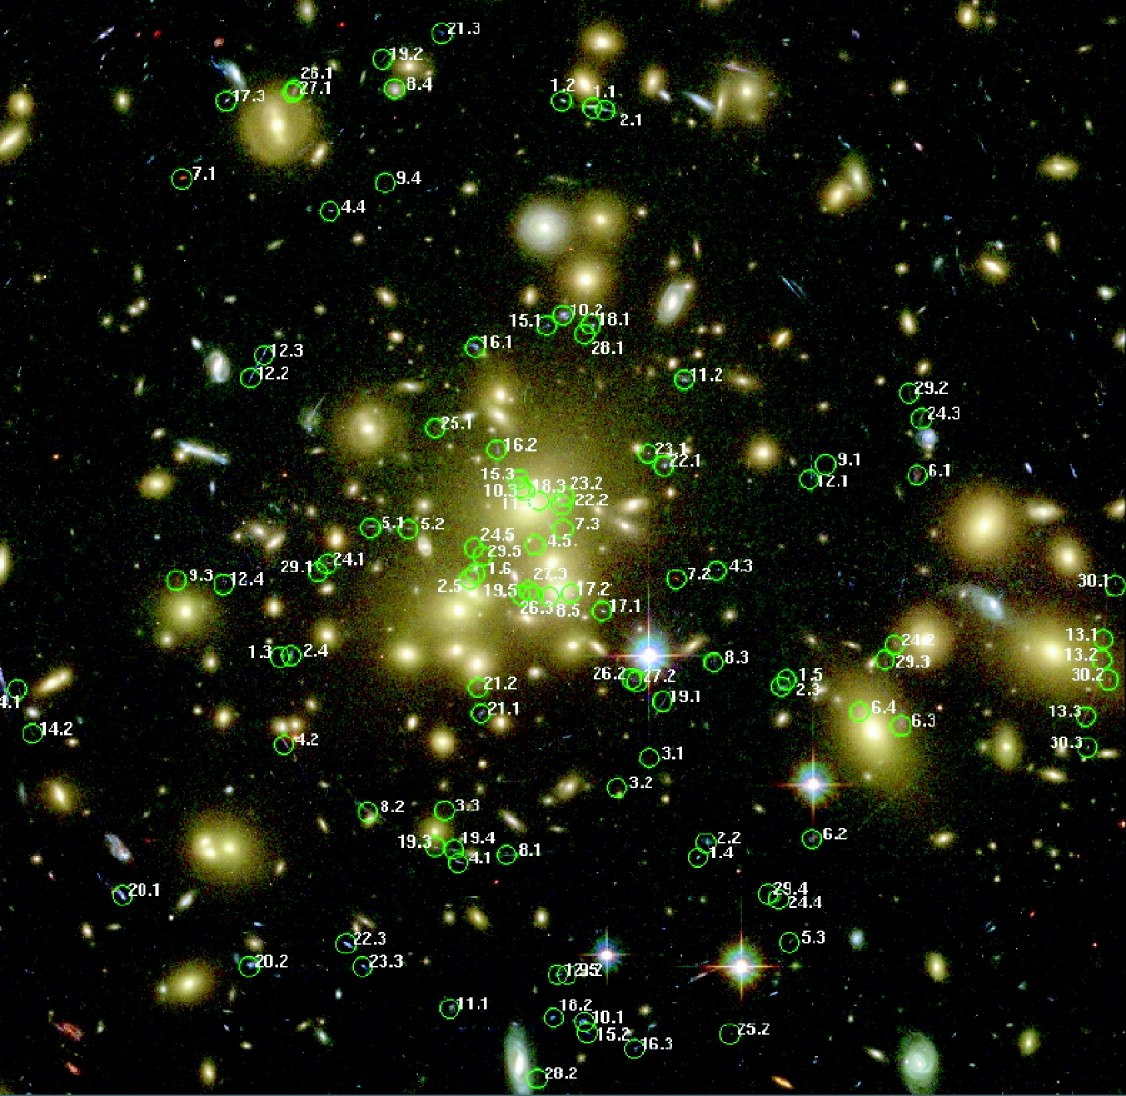
\includegraphics[height=0.3\textheight]{Intro/a1689.jpg}
\caption[Abell 2218 and Abell 1689]{\hst\ imaging of Abell~2218 (left) and Abell~1689 (right).}
\label{intro:fig:lensing_clusters}
\end{figure}

The servicing mission for \hst\ in 2002 gave us the new Advanced Camera for Surveys (ACS), which greatly enhanced optical imaging capabilities. \citet{Broadhurst:2005qy} and \citet{Halkola:2006ss} were able to map the mass distribution in fine detail using over a hundred multiple images of background sources of Abell 1689 with the new ACS data, shown in Figure~\ref{intro:fig:lensing_clusters}. Furthermore, the Wide Field Camera 3 (WFC3) installed during the final servicing mission in 2009 ignited the field of cluster strong lensing with several groups working to develop new lens modeling techniques. This camera has both ultraviolet, optical, and near-infrared imaging sensitivity, allowing for full bandwidth coverage of lensing clusters.

The {\it Spitzer Space Telescope} has also greatly added in the field of cluster lensing. While it cannot achieve the same resolution as \hst, it can greatly help distinguish between foreground and background objects in the field of view with adding data to galaxies' spectral energy distribution (SED) in the far-infrared.

\section{Fantastic lenses and where to find them}

The selection techniques for galaxy clusters exhibiting strong gravitational lensing can generally be split into two categories: ``high mass" and ``high magnification." Galaxy clusters may be selected by mass for lensing, as those more massive will tend to provide a larger cosmological volume for which $\kappa>1$, thus having high cross sections for lensing many background galaxies. However, galaxies need not be massive to lens a single galaxy to a very high magnification ($\mu>30$). The techniques for finding these clusters are different as are their scientific applications.

\subsection{Surveys for finding clusters}

Some of the first cluster lenses were identified in wide-field optical surveys. For example, the Abell clusters \citep{Abell:1958mz,Zwicky:1968rm,Abell:1989ly} were found in large surveys of photographics plates and identified based on the clustering of several massive red galaxies located within a few arcminutes of one another, all with similar photometric colors. Generally speaking, more massive clusters tend to have higher galaxy membership, or ``richness." Abell 1689 and Abell 370, as we discussed earlier, are prime examples. With digitized data, clusters can be found in optical/near-infrared surveys using algorithms aimed at identifying clusterings of close in photometric redshift estimations \citep{Rykoff:2014rz} and by identifying the red sequence of early-type galaxies on a color-magnitude diagram \citep{Gladders:2000kq}.

With the advent of Xray telescopes, more massive clusters were able to be identified. A hot ionized intercluster medium fills the space between galaxies. In order for this gas to maintain hydrostatic equilibrium within the gravitational potential of the cluster, it must be a temperature of order $10^7$ to $10^8$ K, with $M\propto T_X^{3/2}$ based on theoretical arguments for a relaxed system \citep{Horner:1999rz}. Plasmas at this temperature will emit high energy photons on the order of a few keV via thermal bremsstrahlung radiation. Massive clusters ($T>5$ keV) can be targeted and identified as lensing clusters with optical imaging. The Massive Cluster Survey \citep[MACS; ][]{Ebeling:2001rt} carried out this method by applying Xray brightness and hardness cuts to sources in the ROSAT All Sky Survey and cross-matched with optical surveys and follow-up observations to find the most massive galaxy clusters at $z>0.3$. The selection effect for Xray-selected clusters is redshift-dependent as a result of cosmological dimming of the emission.

The hot intercluster medium of also provides a second means for detection. Photons from the cosmic microwave background (CMB) are cooler than the gas surrounding galaxy clusters and can receive an energy boost from inverse Compton scattering. This phenomenon is known as the Sunyaev-Zel'dovich effect. As a result, the CMB photons passing through a galaxy cluster will ``disappear" at the frequencies below the thermal null frequency of the CMB at $\sim220$~GHz and ``reappear" at higher frequencies. Over a thousand clusters have been found in the Planck all-sky survey of the CMB \citep{Planck-Collaboration:2014gf}. More massive clusters will have a stronger CMB detriment, thus the sample is mass-limited. However, the large seven arcminute beam can cause significant beam-dilution for sources with angular sizes smaller than the beam, and therefore also takes a hit at detecting clusters at higher redshifts. Other surveys work with smaller beam sizes and thus, while still mass-limited, are able to push cluster detections out past $z=1$. The most massive galaxy cluster beyond $z=0.87$, nicknamed ``El Gordo" \citep{Menanteau:2012ul, Menanteau:2010fu}, was found along with nearly 100 other clusters by the Atacama Cosmology Telescope \citep[ACT; ][]{Hasselfield:2013pd,Marriage:2011qf}. The South Pole telescope \citep[SPT; ][]{Bleem:2015gf} has detected nearly 900 clusters over a 2500 square degrees. 

\begin{figure}
\centering
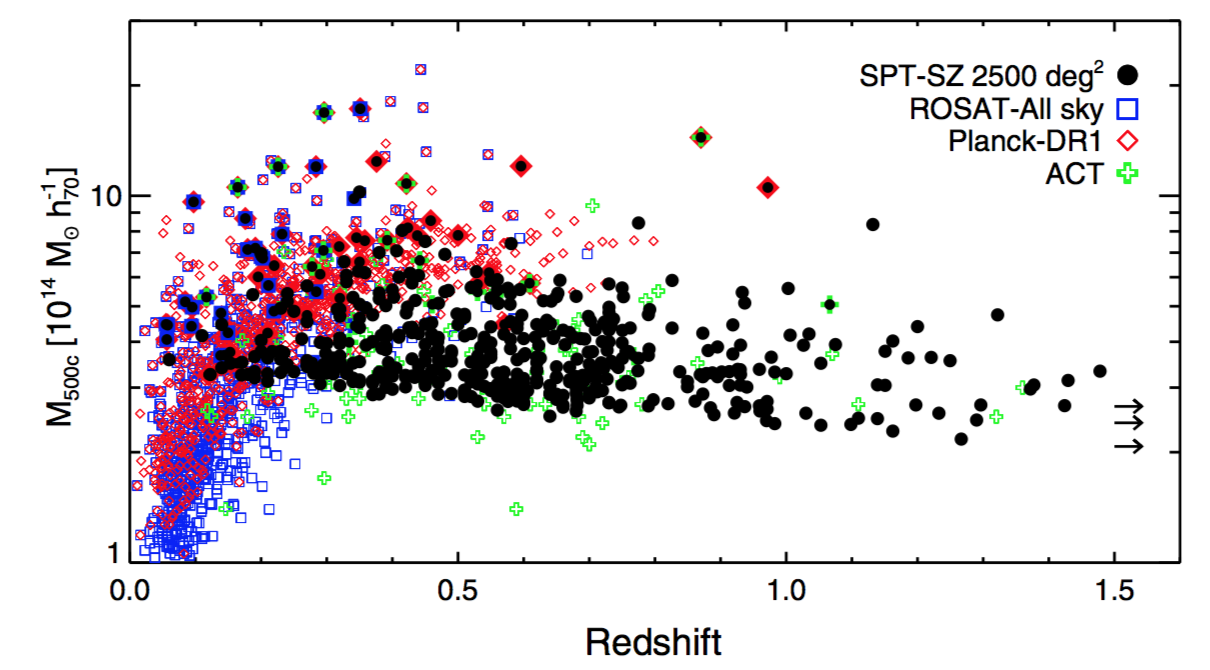
\includegraphics[width=\textwidth]{Intro/spt.png}
\caption[Masses and redshifts of cluster detections]{From \citet{Bleem:2015gf}: The masses and redshifts of optically-confirmed clusters discovered in the SPT, ACT, Planck and ROSAT surveys.}
\label{intro:fig:cluster_detections}
\end{figure}

Figure~\ref{intro:fig:cluster_detections} shows these clusters plotted in mass and redshift. It is important to note that mass is not a direct quantity that any of the methods above can measure. Our best way of measuring the total mass of a galaxy cluster is through weak gravitational lensing, where the integrated surface mass density along the line of sight is measured using the slight distortions in the shapes of background galaxies to map the shear. Since galaxies can intrinsically have elongated shapes, thousands of background sources are needed in order to determine a statistically significant sample for the shear across the entire field of the cluster. Therefore, high-resolution ($<$1"), wide-field (several square degrees) imaging is needed for these measures, as well as accurate estimates for the redshifts of the background sources, in order to eliminate the mass sheet degeneracy \citep{Schneider:1995vn}. The ``Weighing the Giants" project has measured weak lensing mass and systematics for 51 massive clusters based on imaging from both the {\it Subaru} and {\it Canada-France-Hawaii Telescopes} \citep{von-der-Linden:2014wd}, which can be compared with other scaling relations for mass.

\subsection{Discovering galaxies at cosmic dawn}

As mentioned earlier, ``high mass" clusters are the best for finding the most distant galaxies in the Universe. These techniques combine two powerful tools: massive lensing clusters and \hst\ along with deep integrations on the scales of hundreds of orbits. Using lensing can be powerful but makes analysis of determining a luminosity function more difficult. Lensing magnifies not only the sources, but the volume for which galaxies can be significantly magnified. Because of the smaller survey volume, the counts of lower redshift galaxies in lensed fields can be slightly lower than in unlensed fields, like those of Cosmic Assembly Near-infrared Deep Extragalactic Legacy Survey \citep[CANDELS; ][]{Grogin:2011ly} and the Hubble Ultra Deep Field \citep{Beckwith:2006rt}. However, the source plane area for higher redshifts will increase, and with a higher magnification, more galaxies at $z>8$ can be seen. Our best hopes at finding sources with double digit redshifts rely on cluster lensing.

The Cluster Lensing and Supernova Search with {\it Hubble} \citep[CLASH; ][]{Postman:2012lr} used this technique on 20 Xray-selected galaxy clusters and 5 known lensing clusters to be imaged in 16 bands of \hst\ ACS and WFC3. The high photometric resolution allows for more accurate lens modeling, both strong and weak, as well as more accurate photometric redshifts \citep{Jouvel:2014qy}. CLASH provided the means to set more stringent limits on the star formation rate density at $z=9-10$ \citep{Bouwens:2014zp} as well as precise measures of the mass-concentration relationships of the lensing clusters themselves \citep{Merten:2015rz,Meneghetti:2014ys}. Several exciting discoveries were also made: a triply-imaged $z\sim11$ candidate was found lensed by cluster \citep{Coe:2013tg}, a spectroscopically confirmed, quintuply-imaged $z=6.11$ galaxy was found lensed by Abell S1063 \citep{Monna:2014lr,Balestra:2013uq}, and three lensed supernovae at $z=0.85,1.14,1.28$ were discovered \citep{Patel:2014kl}, two of which were Type Ia and could be used to challenge the magnification predictions of the lens models.

In 2013, a director's discretionary time (DDT) proposal was approved for \hst\ over the course of Cycles 22-24 to image 6 massive clusters, 140 orbits each and in 7 ACS and WFC3/IR bands. This survey, the Frontier Fields \citep{Lotz:2017gd} aimed at pushing beyond the limits of CLASH and predicted to yield up to 70 $z>9$ candidates \citep{Coe:2015qf}. As this was a DDT program, the data are publicly available immediately when downloaded from the telescope. Therefore, in efforts to level the playing field for the high redshift community with or without lensing experience, the lens models were also made publicly available (a discussion on this process and the creation of the models is given in Chapter~\ref{chap:hff_clusters} of this dissertation).

\subsection{High-resolution galaxies at cosmic noon}

Finding galaxies lensed to extraordinary magnifications is extremely rare; however, it is possible to find them buried in data sets cataloging thousands of clusters. Scanning through thousands of cut out images of galaxy clusters in optical surveys for the signatures of strong lensing can be a painstakingly tedious process for any individual to endure. But, believe it or not, a lot of dedicated astronomers have carried out this task on data. These projects include the Red Sequence Cluster Survey \citep[RCS;][]{Gladders:2003zr}, the Sloan Giant Arc Survey \citep[SGAS; Gladders~et~al. in preparation, ][see Figure~\ref{intro:fig:gallery}]{Hennawi:2008mz}, SPT optical follow-up \citep{Bleem:2015gf}, and the Dark Energy Survey \citep[DES; ][]{Diehl:2017zh}. Ways of making these tasks less daunting include taking advantage of public interest using citizen science projects like Space~Warps\footnote{https://spacewarps.org/} and by utilizing deep learning algorithms to search large datasets for the signatures of strong lensing \citep{Lanusse:2018zv,Nord:2016kc}.

\begin{figure}
\centering
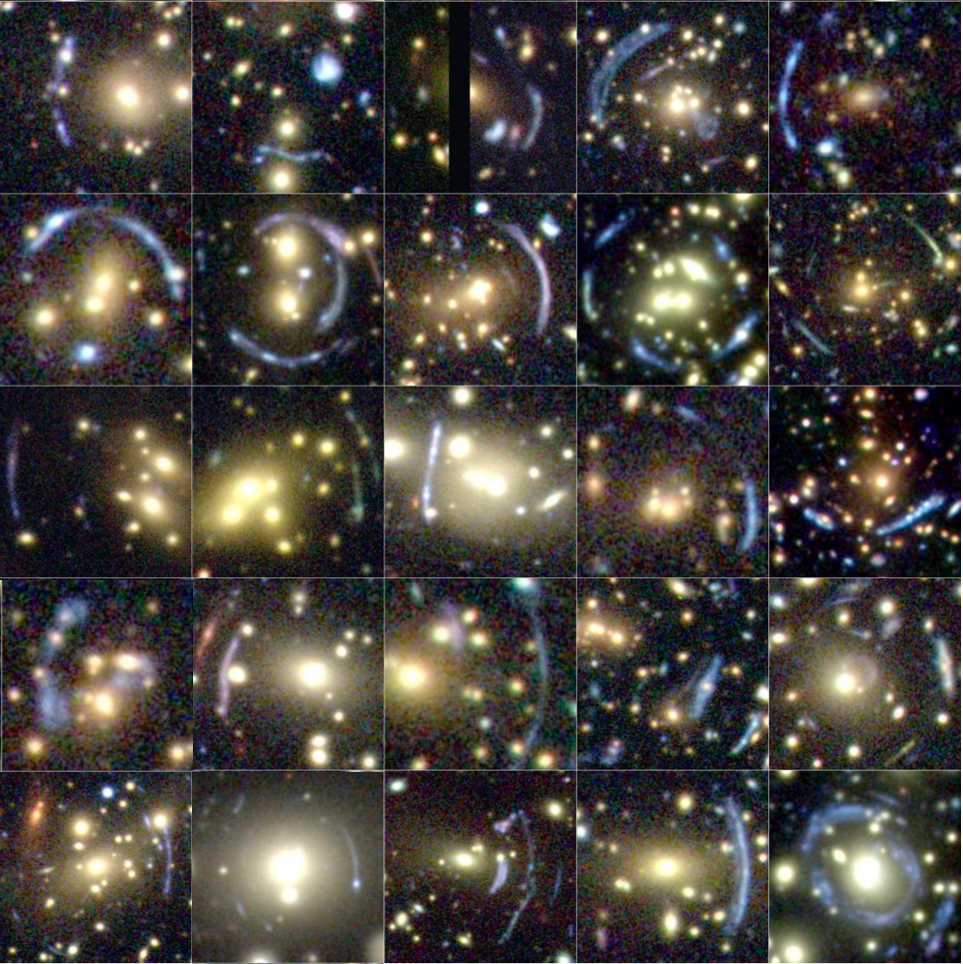
\includegraphics[width=0.8\textwidth]{Intro/gallery.png}
\caption[Gallery of lensing galaxy clusters discovered in SGAS]{A selection of the best lensing clusters found in the Sloan Giant Arc Survey. Each image is $gri$ 5 min exposures with {\it Gemini}/GMOS. Image credit: M.~Bayliss.}
\label{intro:fig:gallery}
\end{figure}

As difficult as it can be to find strong lensing clusters, it is worth it. The hours spent digging through data sets to find higher resolution images of galaxies at $z\sim2$ than in the field pays off in the years, if not decades, of waiting for more powerful telescopes on the ground and in space to be built. Lensing amplifies the sizes of galaxies in the sky by factor of roughly the square root of the magnification, allowing us to peer into the fine details of a galaxy, and even with only a few orbits of \hst\ data. Chapters~\ref{chap:s1110}-\ref{chap:clumps} of this dissertation show an example of how lensing can allow us to break the kiloparsec resolution limit for galaxies at $z\sim2$. 

As we will discuss in the next section, determining an accurate magnification can be difficult and imparts systematic errors into several derived quantities. However, any quantities derived from colors are unbiased because lensing is color-independent. Therefore, lensed galaxies are great laboratories for spectroscopic studies, as observing a single giant arc achieves the same signal-to-noise ratio as a field galaxy in 1/1000th of the exposure time. This allows for a case-by-case study of high redshift galaxies \citep[e.g., ][]{Rigby:2018hs,Rigby:2017yb} rather than relying on stacked spectra from thousands of galaxies \citep[e.g., ][]{Shapley:2003fk}

\section{Systematics of strong lens modeling}

Strong lens modeling of galaxy clusters has come a long way from where it began a little over a decade ago. The earliest models often did not provide any statistical errors as doing so at the time would be extremely computationally intensive. Computing power has greatly increased and nearly all lens modeling codes now implement some version of a Bayesian MCMC to adequately sample the parameter space of a lens model from which calculating statistical errors is trivial.

The Frontier Fields lens models were a great experiment for the lens modeling community in the context of beginning to understand systematics. All the teams constructed models with their own techniques using the same lensing information and their models did not produce the same results. Figure~\ref{intro:fig:hff_models} show the differences in the regions of high magnification for the cluster Abell 2744. These modeling variations were of concern as the systematic errors in magnification across the field of the cluster translate directly to systematics in the derived luminosity functions: both in the corrections for intrinsic source luminosity as well as for the size of the survey volume. This prompted the Frontier Fields lens modeling comparison project \citep{Meneghetti:2016xe}, where several lens modeling softwares were put to the challenge of modeling two simulated clusters ``observed" through the eyes of \hst\ to the same depths as the Frontier Fields. The models produced reliable mass models of the clusters, likely as a result of the many multiple images and constraints with full knowledge of the source redshifts provided. This test was reassuring as the Frontier Fields lens models, with full depth data and several spectroscopic campaigns, are less vulnerable to systematics.

\begin{figure}
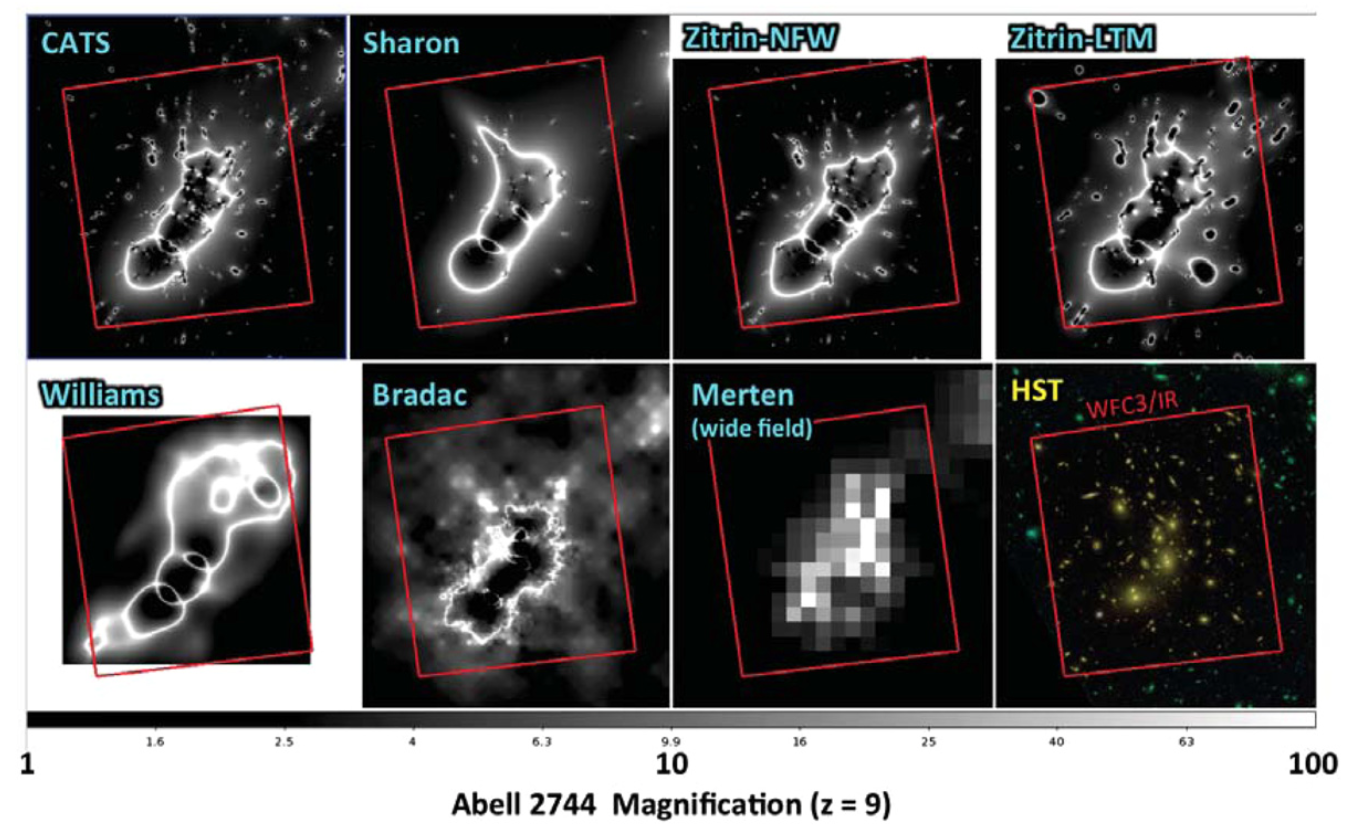
\includegraphics[width=\textwidth]{Intro/hff_models.png}
\caption[Magnification maps of Abell~2744 produced by Frontier Fields lens modeling teams]{From \citet{Coe:2015qf}, original caption: ``Magnification maps (log grayscale) for $z=9$ galaxies lensed by A2744 according to all seven submitted gravitational lensing models. The Frontier Fields WFC3/IR FOV (136"$\times$123") is outlined in red. At bottom right is a color HST image \citep[produced with Trilogy; ][]{Coe:2012px} showing the Frontier Fields WFC3/IR observations (red channel) within the prior ACS observations (blue-green). North is up and East is to the left."}
\label{intro:fig:hff_models}
\end{figure}

It is clear, though, that there was significant systematic error in the lens models of the Frontier Fields produced prior to when the data were taken. These models were built with far few constraints and many only had a few spectroscopic redshifts of the background galaxies. Therefore, a major source of the systematics is in the selection of constraints themselves. The systematic errors in mass and magnification for a cluster like those of the Frontier Fields benefit from increased numbers of constraints and redshifts. However, there is a point where the global systematic errors begin to saturate and are likely a product of the positions and redshift distributions of the constraints themselves. Areas in the image plane where constraints are nearby will have lower statistical and systematic errors, especially if the redshift of that source galaxy is known. This will be discussed further in Chapter~\ref{chap:ares_systematics} and Chapter~\ref{chap:sim}.

\section{Dissertation overview}

This dissertation consists of five chapters demonstrating the use of strong gravitational lens modeling to study the high redshift universe, as well as how to better understand and improve our methods when it comes to systematic errors.

Chapter~\ref{chap:hff_clusters} describes the lens models of the six Frontier Fields clusters. These models were created in 2014 using on archival \hst\ imaging supplemented by ground-based spectroscopic observations, including some provided within this chapter. The Frontier Fields lens models created by this author are in addition to several others created using various other lens modeling techniques, all of which are publicly available to the users of the Frontier Fields data sets.

Chapter~\ref{chap:ares_systematics} begins to quantify the systematics involved in this author's lens modeling techniques based on constraint selection and redshift information. Hundreds of lens models of the simulated cluster Ares were realized using different numbers of images and varying levels of precision for the redshift information of the sources. Therefore, we were able to quantify the dependency of errors on mass, magnification, and image plane scatter as they relate to the availability of constraints.

Chapter~\ref{chap:s1110} provides a full lensing analysis of the cluster \cluster. It begins with a description of the hybrid lens modeling technique used to model the mass of the cluster. Then, a forward modeling technique is described and implemented on the giant arc \giantarc\ to create a source plane reconstruction of the source galaxy.

Chapter~\ref{chap:clumps} builds on the previous chapter's source plane reconstruction to report both the sizes and star formation rates of the clumps within the galaxy. These clumps are then compared to the literature, showing an unprecedented level of resolution compared to field galaxies and other source plane reconstructions of lensed galaxies using different methods.

Chapter~\ref{chap:sim} looks briefly at quantifying the systematic errors in a simulated galaxy cluster not all that different from \cluster, where there are very few constraints and spectroscopic redshifts. We will investigate the effects of adding more spectroscopic redshifts changes the systematic errors in both mass and magnification.

Chapter~\ref{chap:future} provides insight into the future directions of lens modeling in ``the era of precision lensing", where our lens modeling techniques are sophisticated and we have now the computational power to compute the statistical errors on quantities on the levels of a few percent. Fully quantifying systematic errors in the realm of clusters with few constraints and redshifts will be vital in the era of large surveys to come.






